%----------------------------------------------------------------------------------------
%	PACKAGES AND THEMES
%----------------------------------------------------------------------------------------
\PassOptionsToPackage{table}{xcolor}
\documentclass[aspectratio=169,xcolor=dvipsnames,svgnames,x11names,fleqn]{beamer}
% \documentclass[aspectratio=169,xcolor=dvipsnames,fleqn]{beamer}

\usetheme{RedVelvet}

\usefonttheme[onlymath]{serif}



\usepackage{xspace}
\usepackage{amsmath}
\usepackage{amssymb}
\usepackage{amsfonts}
\usepackage{color}
\usepackage{physics}
% \usepackage{mathbb}
\usepackage{rahul_math}
\usepackage{bigints}
\usepackage{hyperref}

\usepackage{graphicx} % Allows including images
\usepackage{booktabs} % Allows the use of \toprule, \midrule and \bottomrule in tables
\usepackage{tikz,pgfplots}
\usepackage{subfigure}
\usetikzlibrary{arrows}
\usepackage{minted}
\definecolor{LightGray}{gray}{0.9}
\definecolor{cream}{rgb}{0.92, 0.9, 0.55}
\definecolor{lightblue}{rgb}{0.68, 0.85, 0.9}


\usepackage{xcolor-material}
\usetikzlibrary{fit}
\tikzset{%
apple/.pic={
  \fill [MaterialBrown] (-1/8,0)  arc (180:120:1 and 3/2) coordinate [pos=3/5] (@)-- ++(1/6,-1/7)  arc (120:180:5/4 and 3/2) -- cycle;
  \fill [MaterialLightGreen500] (0,-9/10)  .. controls ++(180:1/8) and ++(  0:1/4) .. (-1/3,  -1) .. controls ++(180:1/3) and ++(270:1/2) .. (  -1,   0) .. controls ++( 90:1/3) and ++(180:1/3) .. (-1/2, 3/4) .. controls ++(  0:1/8) and ++(135:1/8) .. (   0, 4/7)
}
}

\newcommand{\leftdoublequote}{\textcolor{blue}{\scalebox{3}{``}}}

\newcommand{\rightdoublequote}{\textcolor{blue}{\scalebox{3}{''}}}


\usepackage{textcomp}
\usepackage{fontawesome}

\usepackage{overpic}

%----------------------------------------------------------------------------------------
%	TITLE PAGE
%----------------------------------------------------------------------------------------

\usepackage{tikz-qtree,tikz-qtree-compat}
\usetikzlibrary{calc}


\title[CPE 381: Signals and Systems]{CPE 381: Fundamentals of Signals and Systems for Computer Engineers} % The short title appears at the bottom of every slide, the full title is only on the title page
\subtitle{01 Introduction and Preliminaries}

\author[Rahul Bhadani] {{\Large \textbf{Rahul Bhadani}}}

\institute[UAH] % Your institution as it will appear on the bottom of every slide, maybe shorthand to save space
{
    Electrical \& Computer Engineering,  The University of Alabama in Huntsville
}
\date

% \titlegraphic{
%    \includegraphics[width=0.4\linewidth]{figures/UAH_primary.png}
% }

\begin{document}

%-------------------------------------------------
\begin{frame}
  \titlepage
\end{frame}

%-------------------------------------------------
\begin{frame}{Outline}
   \tableofcontents
\end{frame}

%%%%%%%%%%%%%%%%%%%%%%%%%%%%%%%%%%%%%%%%%%%%%%%%%%%%%
\section{Course Logistics}

%-----------------------------------------.-------
\begin{frame}{About Me}
    \begin{columns}[c] % The "c" option specifies centered vertical alignment while the "t" option is used for top vertical alignment

        \column{.60\textwidth} % Left column and width
        \textbf{Rahul Bhadani} \\
        Assistant Professor \\
        Electrical and Computer Engineering \\
        The University of Alabama in Huntsville \\
        Office: 217-H \\
        Email: {\color{MediumRed}{rahul.bhadani@uah.edu}} \\
        Web: {\color{MediumRed}\url{https://rahulbhadani.github.io/}}

        \column{.30\textwidth} % Right column and width
        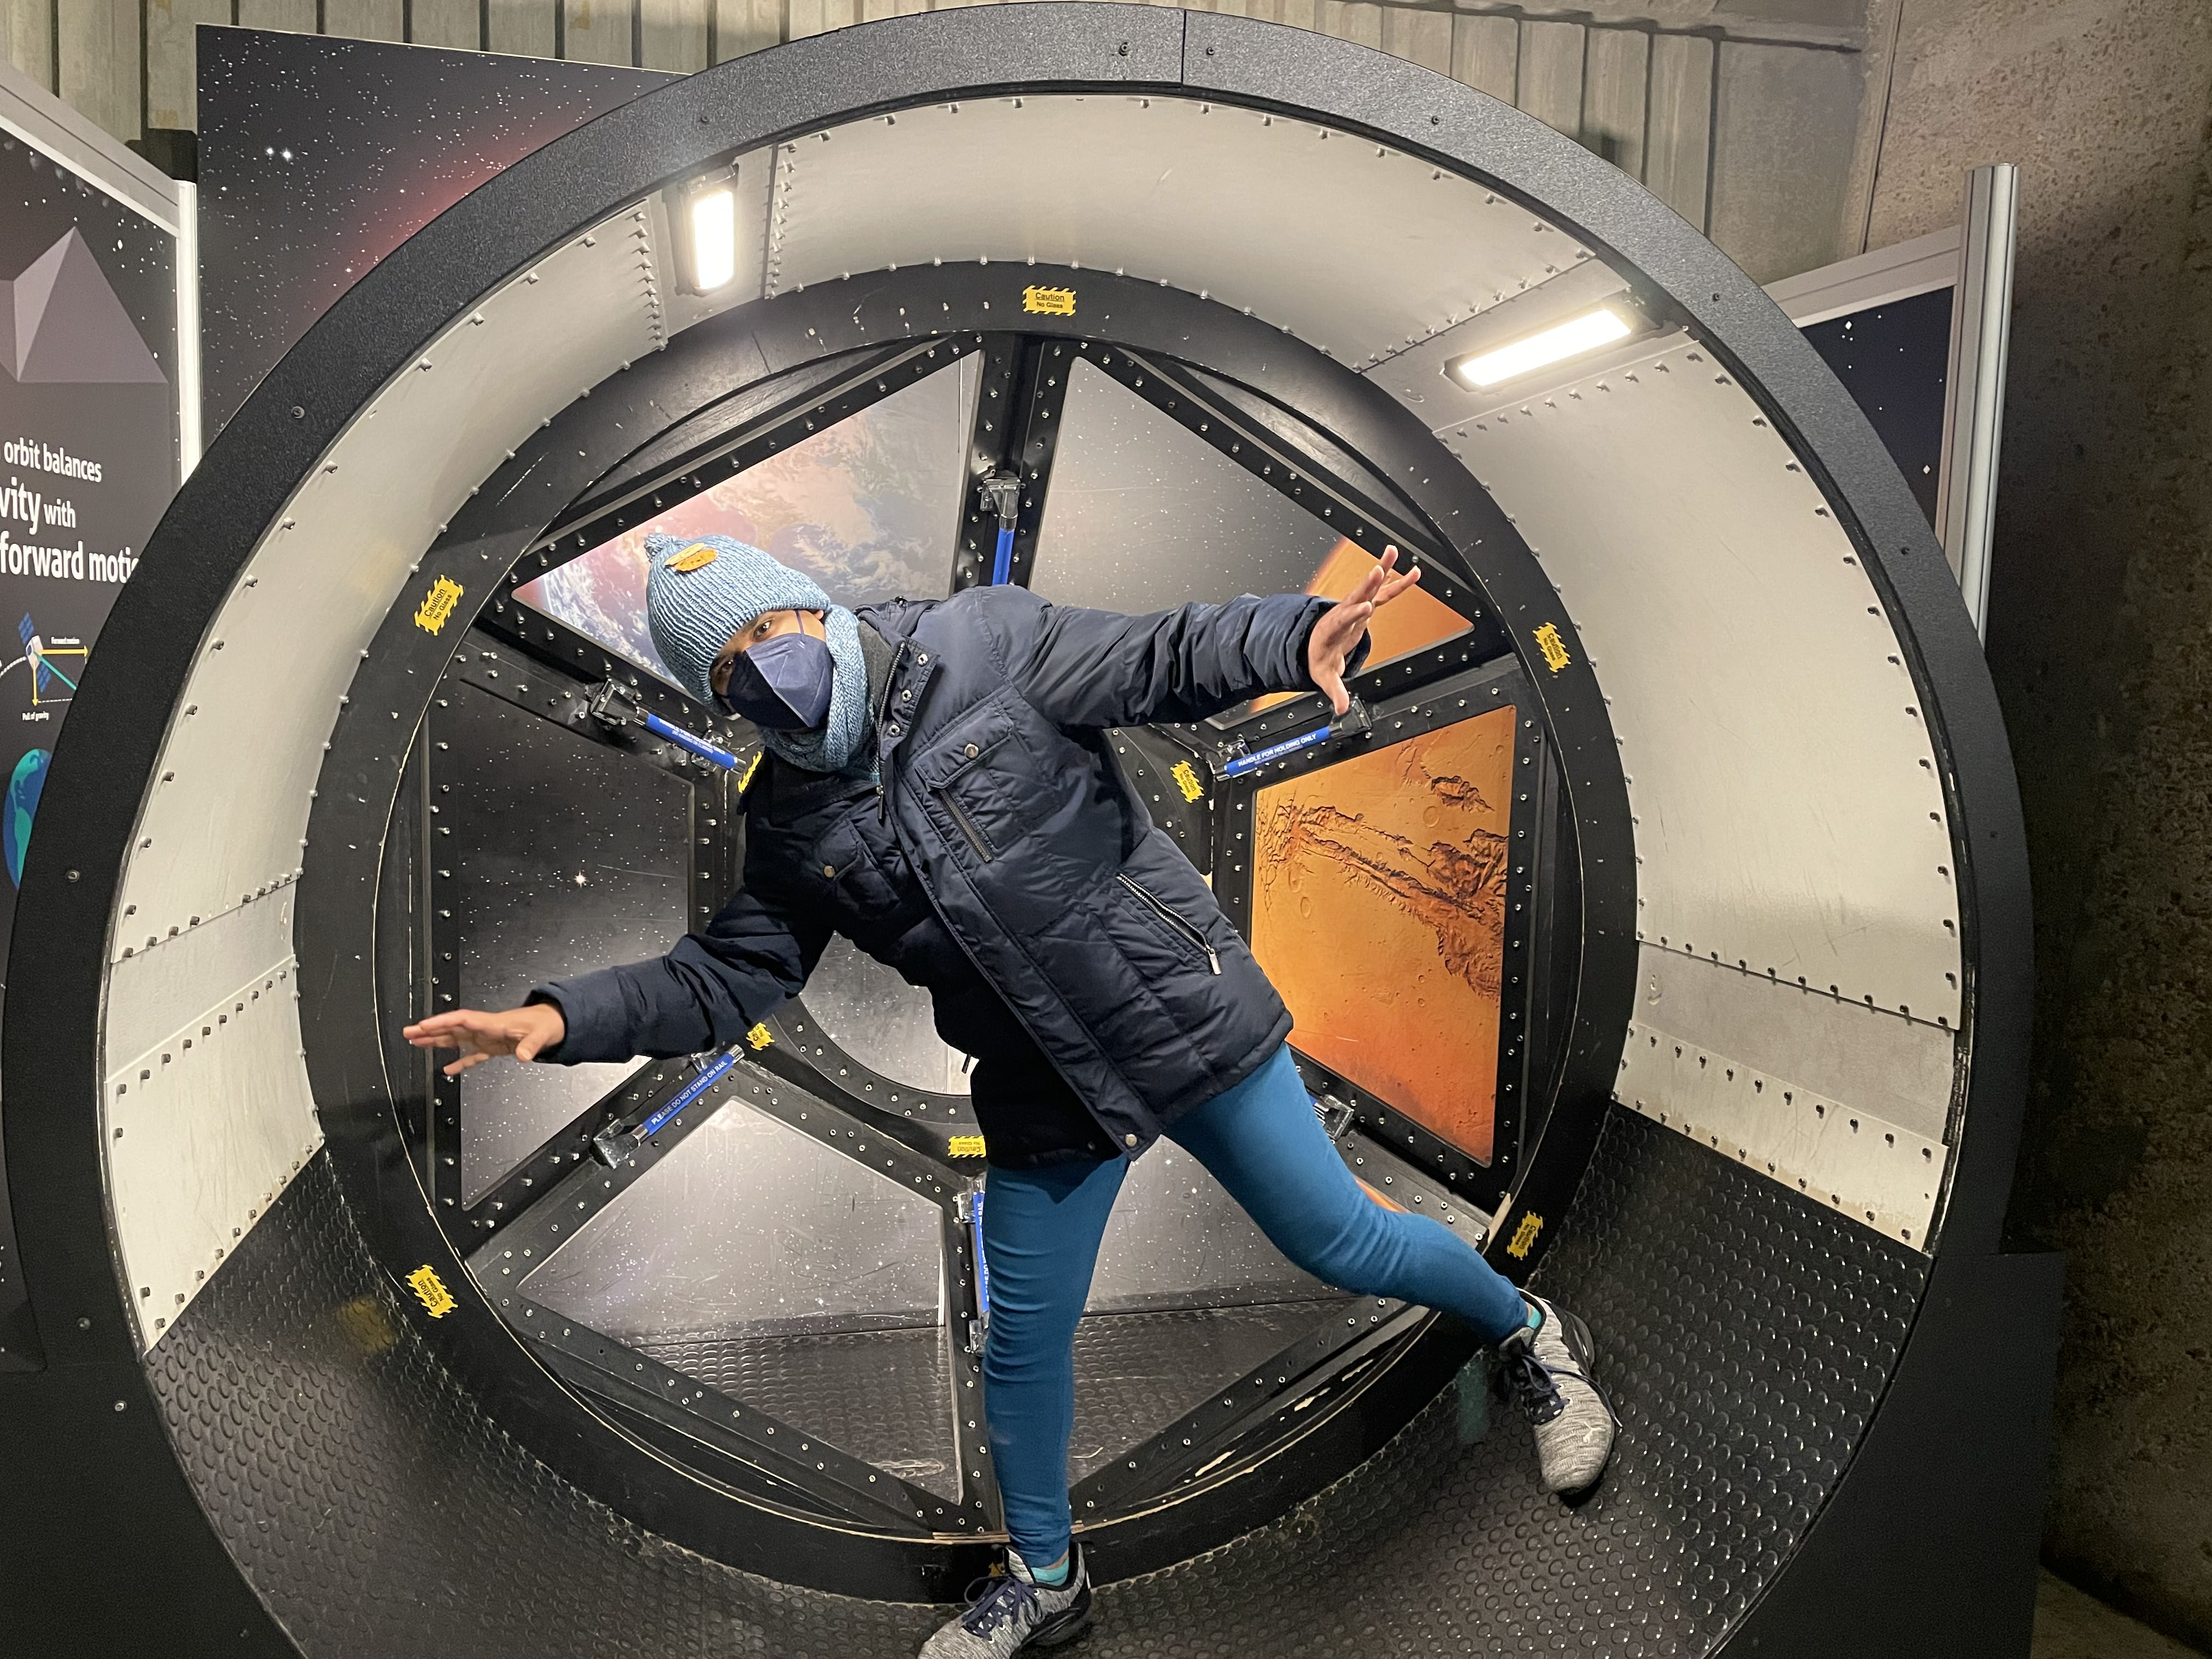
\includegraphics[width=.89\textwidth]{figures/intro_rkb.jpg}
    \end{columns}
    
    \begin{block}{Research Interests}
    Cyber-physical Systems,
    Intelligent Transportation, 
    Connected-and-Autonomous Driving, 
    Applied machine learning,
    Quantum Information Science
    \end{block}
\end{frame}


%-------------------------------------------------

\begin{frame}{Course Logistics
}
  \begin{columns}[T] % align columns at the top
    \begin{column}{0.5\textwidth}
      \textbf{Lecture:} \\
      M/W 11:20 AM - 12:40 PM \\
      \vspace{0.3cm}
      \textbf{Location:} \\
      TBD \\
      \vspace{0.3cm}
      \textbf{Prerequisites:}
      \begin{itemize}
        \item EE 213 - Electrical Circuit Analysis I
        \item MA 238 – Applied Differential Equations
      \end{itemize}
    \end{column}
    \begin{column}{0.5\textwidth}
      \textbf{Office Hours:}
      \begin{itemize}
        \item TBD
      \end{itemize}
      \textbf{Instructor Email:} rahul.bhadani@uah.edu
    \end{column}
  \end{columns}
\end{frame}

%-----------------------------------------
\begin{frame}{Textbooks}
    \underline{Required:} \emph{\color{DarkGreen}Signals and Systems using Matlab}. Luis F. Chaparro. \par{\color{DarkRed}Elsevier, 3rd Edition, 2019}. \par ISBN: 978-0-12-814204-2, eBook ISBN: 9780128142059\par\vspace{5pt}

        \underline{Suggested Reading:} \textit{Linear Systems and Signals}, B. P. Lathi, Roger Green, Oxford University Press, 2017, 3rd Edition

        \underline{Other Notable Textbooks:}
        \begin{itemize}
            \item Schaum's Outline of Signals and Systems
            \item \textit{Signals and Systems}. Haykin, Simon, and Barry Van Veen. John Wiley \& Sons, 2007.
            \item Asadi, Farzin. Signals and Systems with MATLAB and Simulink. Springer, Dec 2023. ISBN: 9783031456220, 303145622X
        \end{itemize}
\end{frame}

%-----------------------------------------
\begin{frame}{Grading}
\begin{columns}
    \column{0.6\linewidth}

\begin{tabular}{lp{1in} l l l}
\textbf{Homework:} & 20\% \\
 \textbf{Quizzes:} &  5\%\\
\textbf{Attendance/In-Class Participation:} & 15\%\\
\textbf{Mid-term Exam 1:} & 15\%  \\
\textbf{Mid-term Exam 2:} & 15\%  \\
\textbf{Final Exam:} & 30\%  \\
\end{tabular}
\column{0.4\linewidth}
\begin{tabular}{|p{3cm}|p{1.5cm}|}
\hline
\multicolumn{2}{|c|}{\textbf{Grading Scale}} \\ \hline
\textbf{Percentage} & \textbf{Grade} \\ \hline
90\% - 100\% & A \\ \hline
75\% - 89\% & B \\ \hline
60\% - 74\% & C \\ \hline
45\% - 59\% & D \\ \hline
0\% - 44\% & F \\ \hline
\end{tabular}
\end{columns}
\end{frame}


\begin{frame}{Homework Policy}
\begin{itemize}
\item Each late submission will be penalized by 10\% per day for up to 5 days maximum, thereafter, if later, one will receive 0 credit. 
\item Solution to homework will be posted 5 days after the due date.
\end{itemize}

\end{frame}

\begin{frame}{Classwork}

\begin{itemize}
\item Each lecture will be followed by in-class problem-solving that students will turn in the next lecture day. If you miss the lecture day (either the day it is handed to you, or the day you need to turn in), you will not receive any credit.

\item There will be intermediate small tests to assess your skills based on lectures and the classwork. This portion will count towards your classwork credits.
\end{itemize}



\end{frame}

\begin{frame}{Attendance Policy}

\begin{itemize}
\item Must attend all lectures.
\item Two unexcused absences permitted.
\item No option to make up for classwork.
\end{itemize}

\end{frame}

%-----------------------------------------
\begin{frame}{Exam Schedule}
\begin{itemize}
\item \textbf{Mid Term 1:}  September 29, Monday
\item \textbf{Mid Term 2:}  November 10, Monday
\item \textbf{Final Exam:}  December 12, Friday
\end{itemize}
\end{frame}

%-----------------------------------------
\begin{frame}{Tentatative Topics}
\small
\begin{itemize}
	\item \color{DodgerBlue4} \underline{Introduction, Mathematical Preliminaries}
 
    \item \color{Firebrick3} \underline{Continuous and Discrete Signals} 
    
    \item  \color{DodgerBlue4} \underline{Linear-time Invariant (LTI) Systems}
    
    \item   \color{Firebrick3} \underline{Laplace Transform}
    
    \item  \color{DodgerBlue4} \underline{Fourier Series for Frequency Analysis} 


    \item  \color{Firebrick3} \underline{Fourier Transform} 
    
    \item \color{DodgerBlue4} \underline{Sampling Theory} 
    \item   \color{Firebrick3}  \underline{Discrete-Time Signals and Systems}
    
    \item  \color{DodgerBlue4} \underline{Z-transform}
    \item  \color{Firebrick3} \underline{Discrete Fourier Analysis} 
   
\end{itemize}
\begin{center}
    Refer to the syllabus for the detailed information on the syllabus.
\end{center}
\end{frame}

%-----------------------------------------
\begin{frame}{In-Class Activity}
  \centering
  \textbf{Introduce Yourself} \\[1em]
  
  \begin{block}{}
    \begin{itemize}
      \item Why Computer Engineering?
      \item Why do you want to take this course?
      \item What is your favorite Pokemon?
    \end{itemize}
  \end{block}

\end{frame}

%%%%%%%%%%%%%%%%%%%%%%%%%%%%%%%%%%%%%%%%%%%%%%%%%%%%%
\section{Motivation}

%-----------------------------------------

\begin{frame}{}
    \begin{center}
    \Huge \bf \color{DarkBlue}
    \faFire
    
    Motivation
\end{center}
\end{frame}

%-----------------------------------------

\begin{frame}{Why Study Signals and Systems}
\centering
    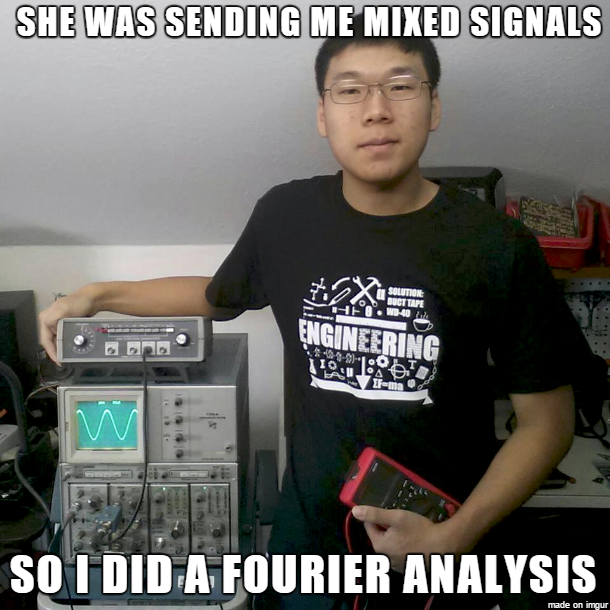
\includegraphics[width=0.4\linewidth]{figures/motivation.png}
\end{frame}

\begin{frame}{We are in digital era}
\centering
    \begin{columns}
          \column{0.33\linewidth}
          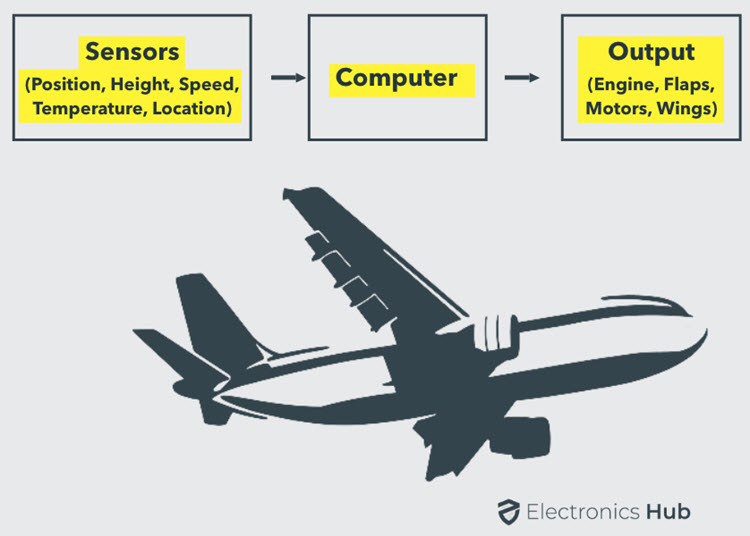
\includegraphics[width=0.99\linewidth]{figures/Types-of-Sensors-in-Auto-Pilot.jpg}
         \column{0.33\linewidth}
          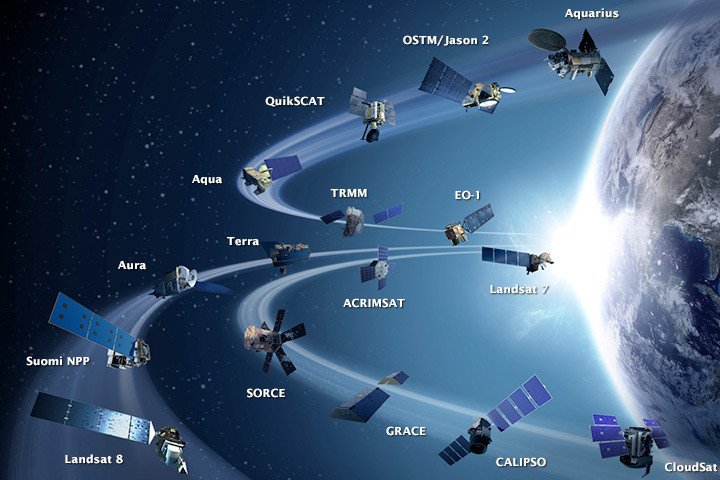
\includegraphics[width=0.99\linewidth]{figures/EarthSat_HD.jpg}
          \column{0.33\linewidth}
          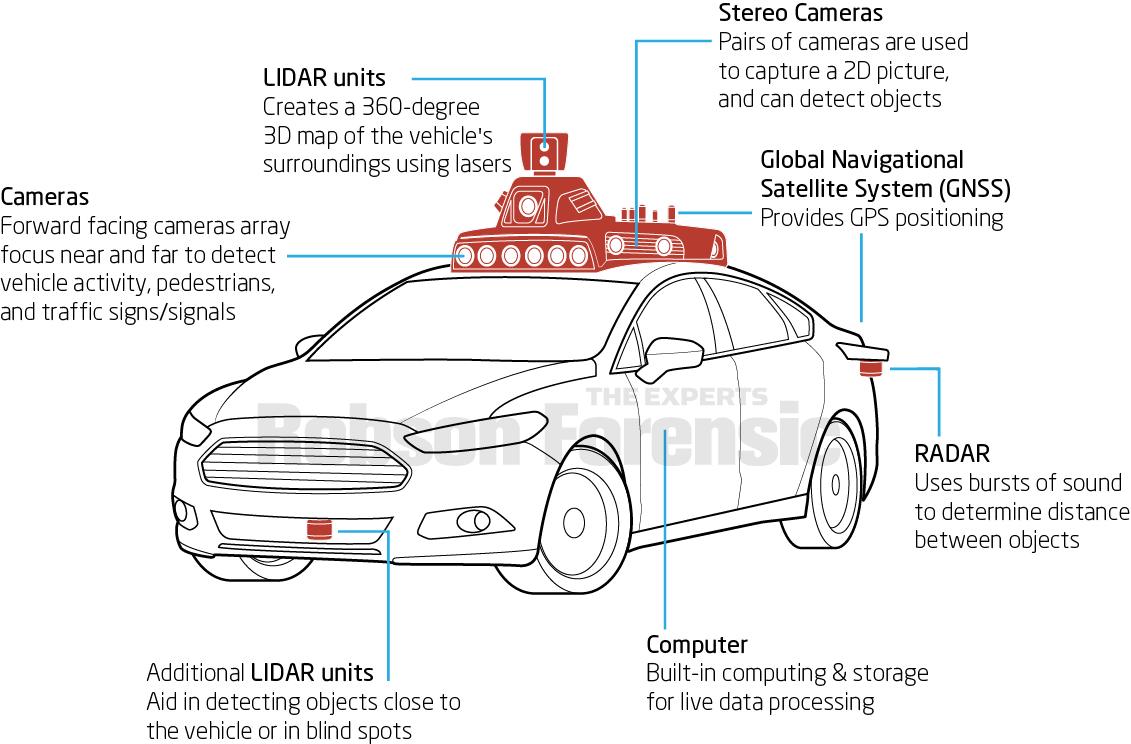
\includegraphics[width=0.99\linewidth]{figures/avsensors.png}
    \end{columns}
\end{frame}


\begin{frame}{Sensors and Mobile Devices}
\centering
    \begin{columns}
          \column{0.66\linewidth}
          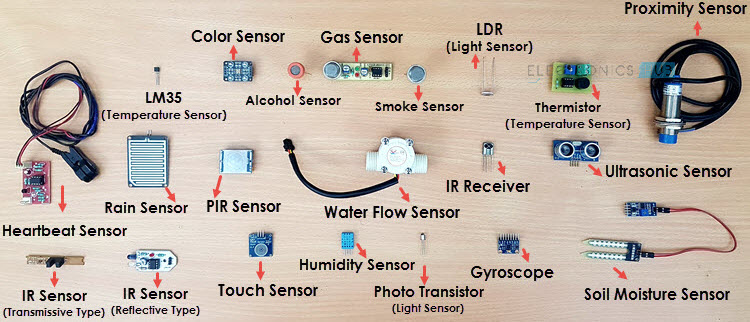
\includegraphics[width=0.99\linewidth]{figures/Types-of-Sensors-Image-2.jpg}
         \column{0.33\linewidth}
          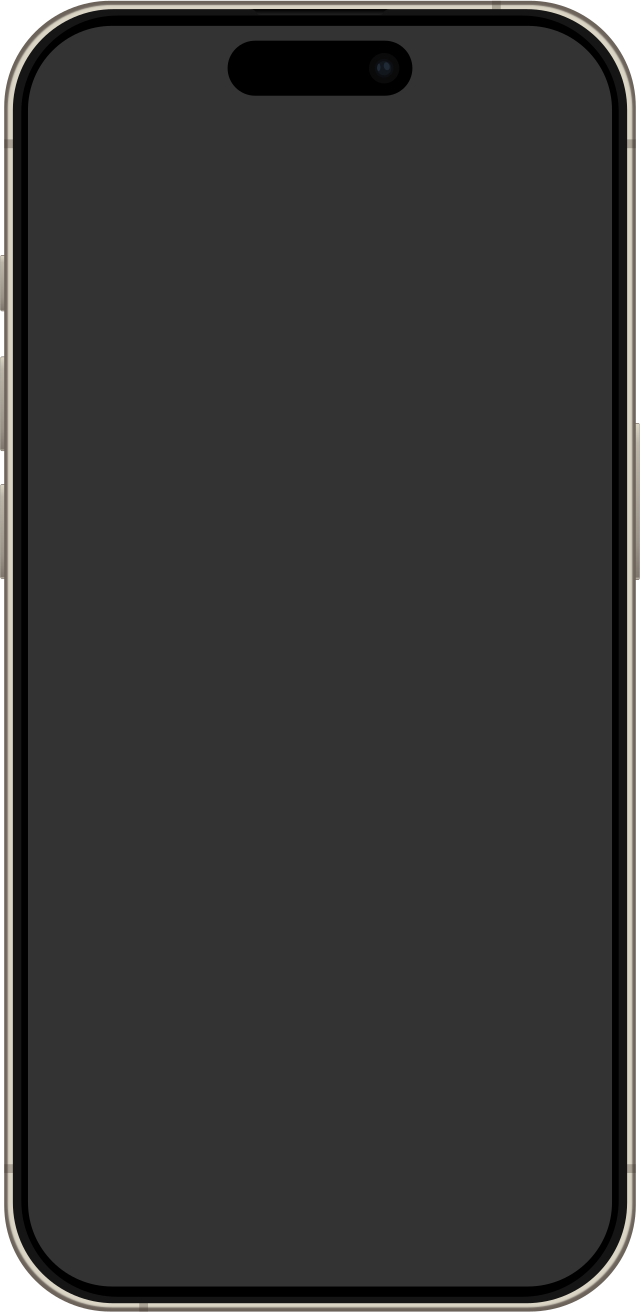
\includegraphics[width=0.6\linewidth]{figures/iphone.png}
    \end{columns}
\end{frame}

\begin{frame}{Cyber-physical Systems}
\centering
    \begin{columns}
          \column{0.45\linewidth}
          \centering
          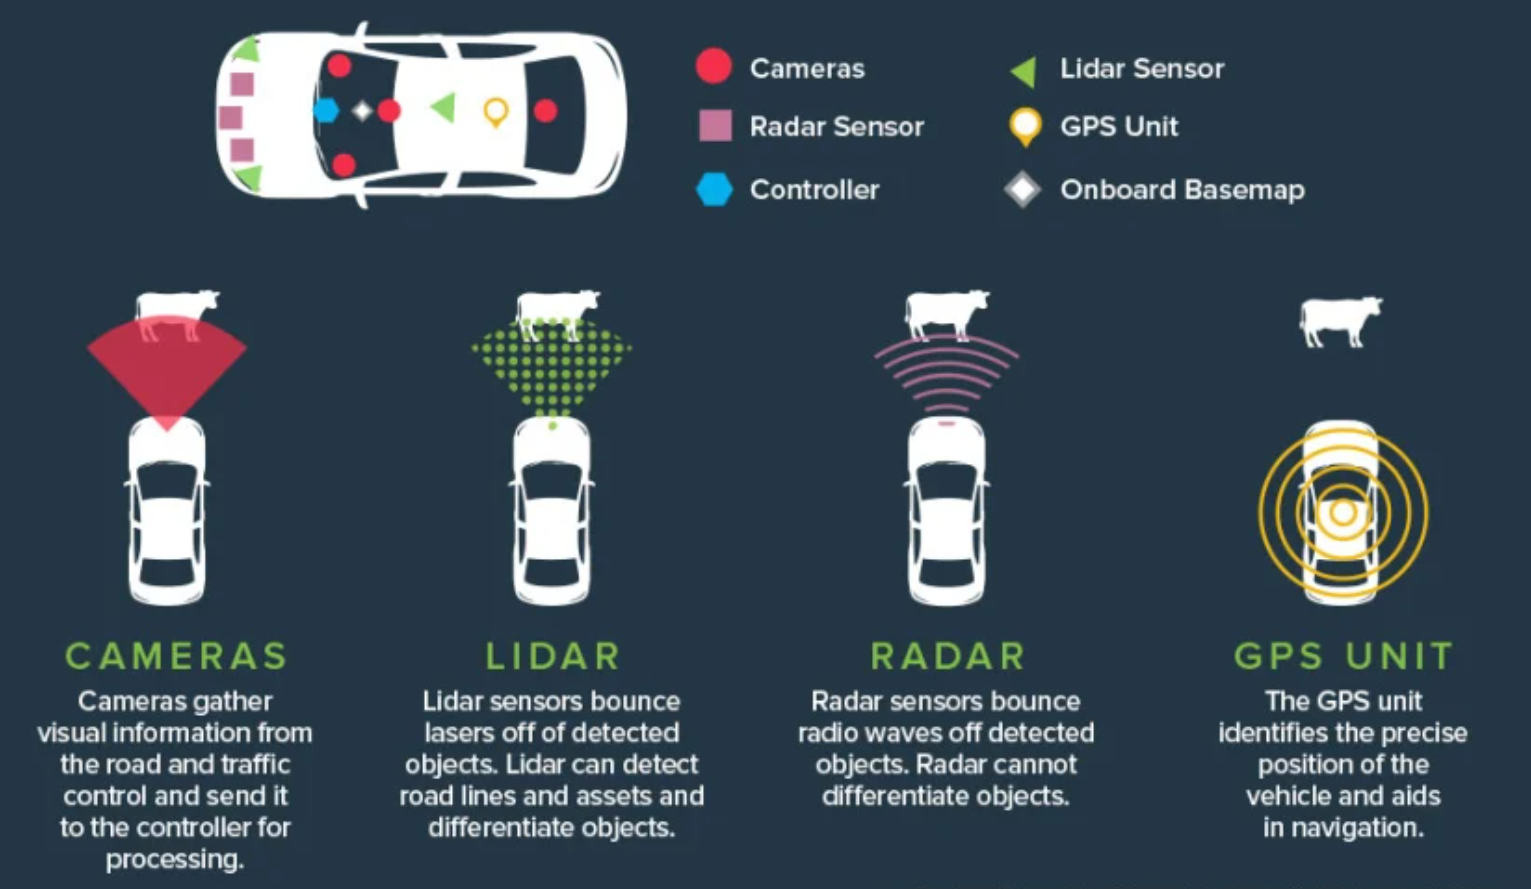
\includegraphics[width=0.99\linewidth]{figures/CPS1.png}
          Connected and Autonomous Vehicles
         \column{0.55\linewidth}
         \centering
          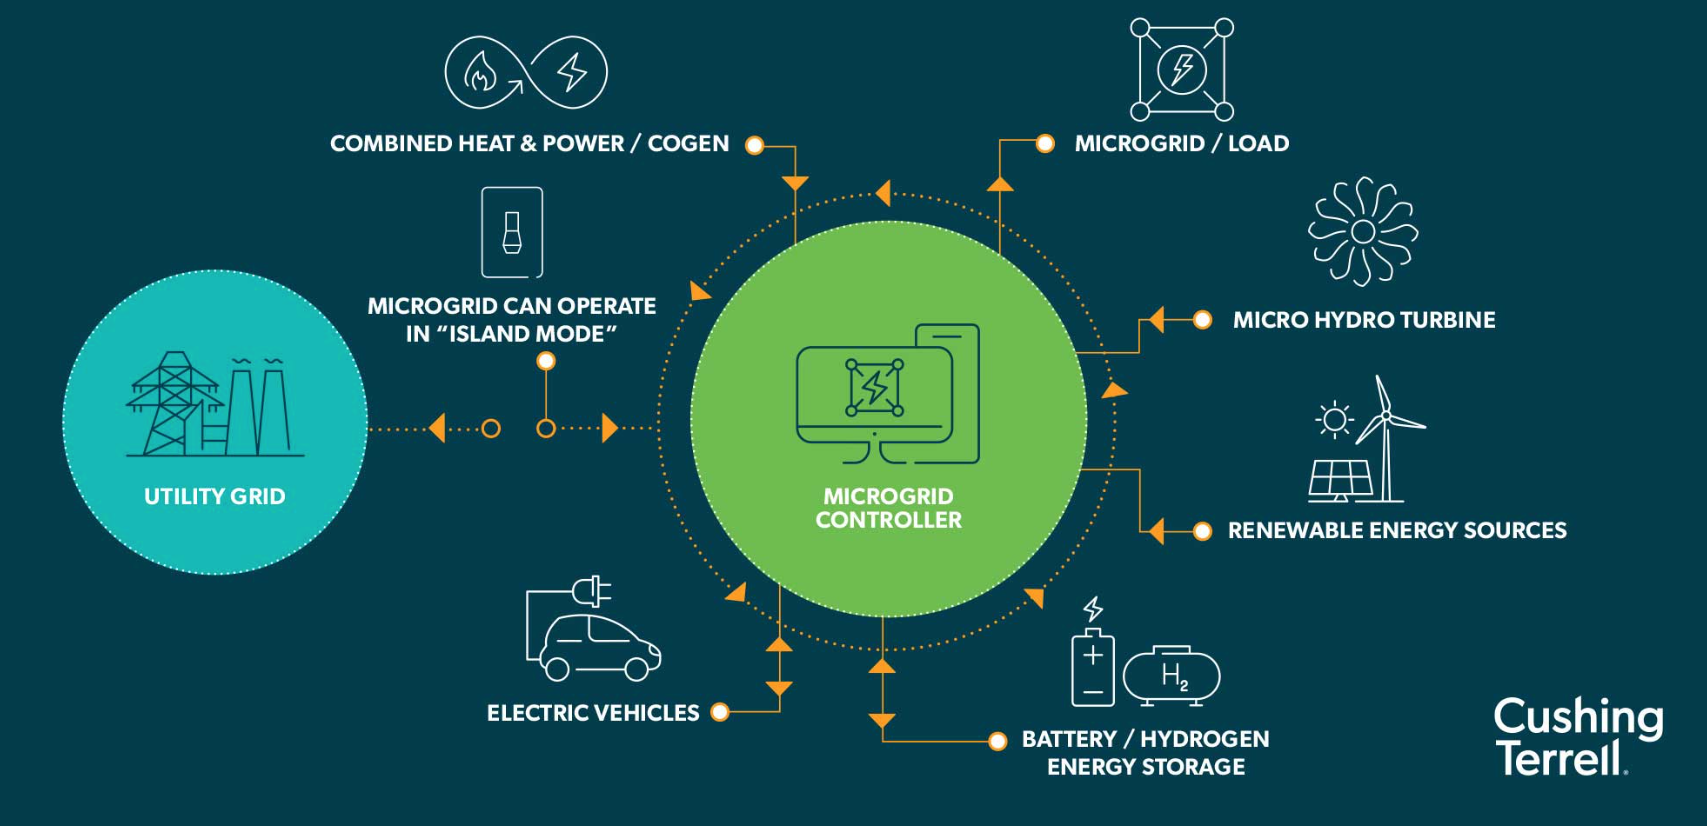
\includegraphics[width=0.99\linewidth]{figures/CSP2.png}
          Microgrid
    \end{columns}
\end{frame}

\begin{frame}{Signals in Nature}
    \begin{center}
        Everything in nature is analog and continuous. We use hardware/software interfaces to digitize them, extract information, make inferences, and send them back to the user.
        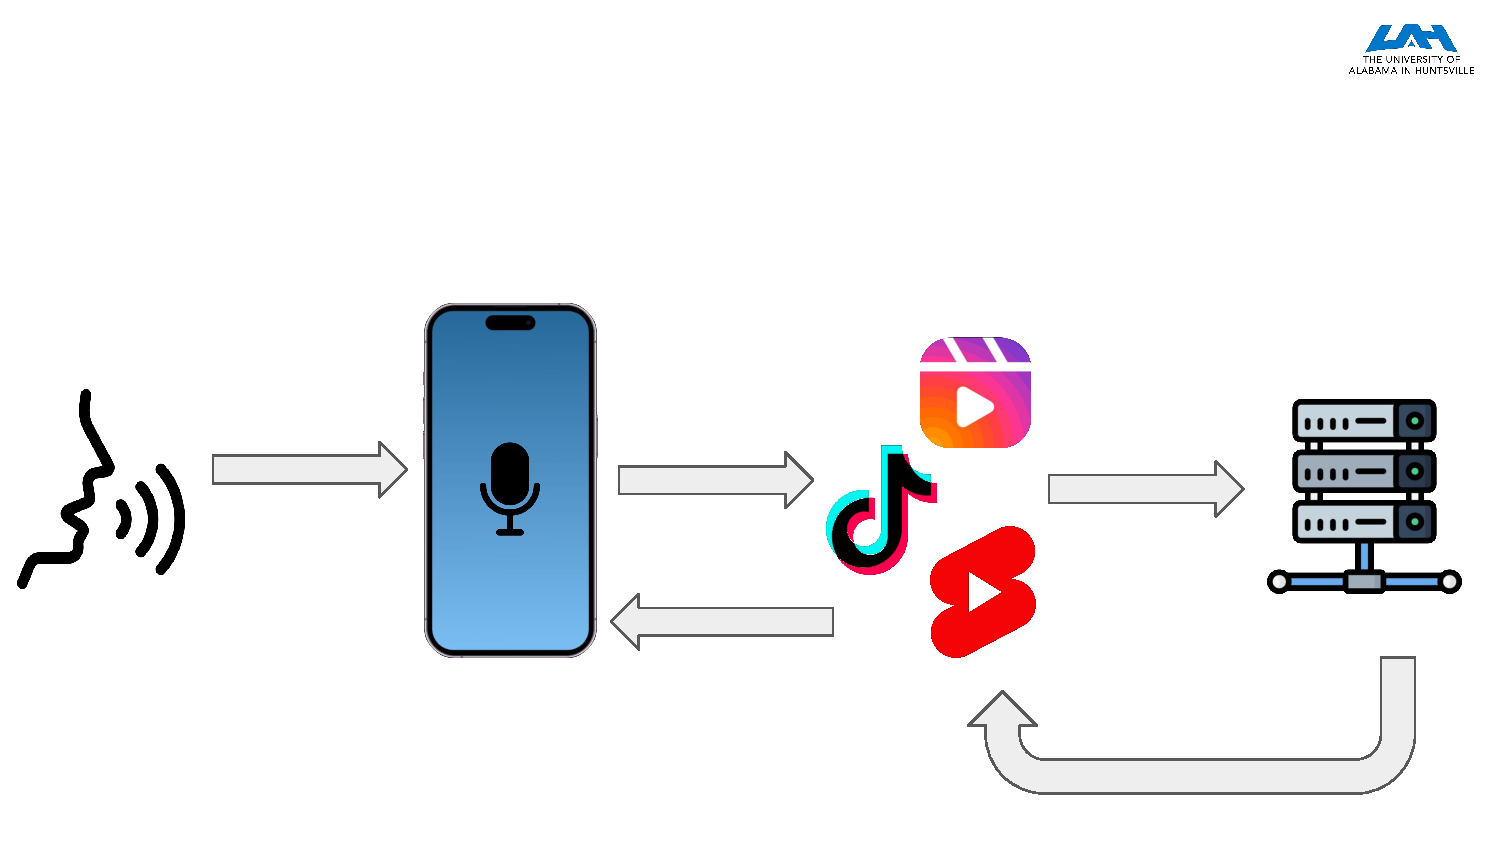
\includegraphics[width=0.95\linewidth, trim=0 0 0 4cm,clip]{figures/signals_comm.pdf}

    \end{center}
\end{frame}

\begin{frame}{Sampling continuous time signals}
\centering
    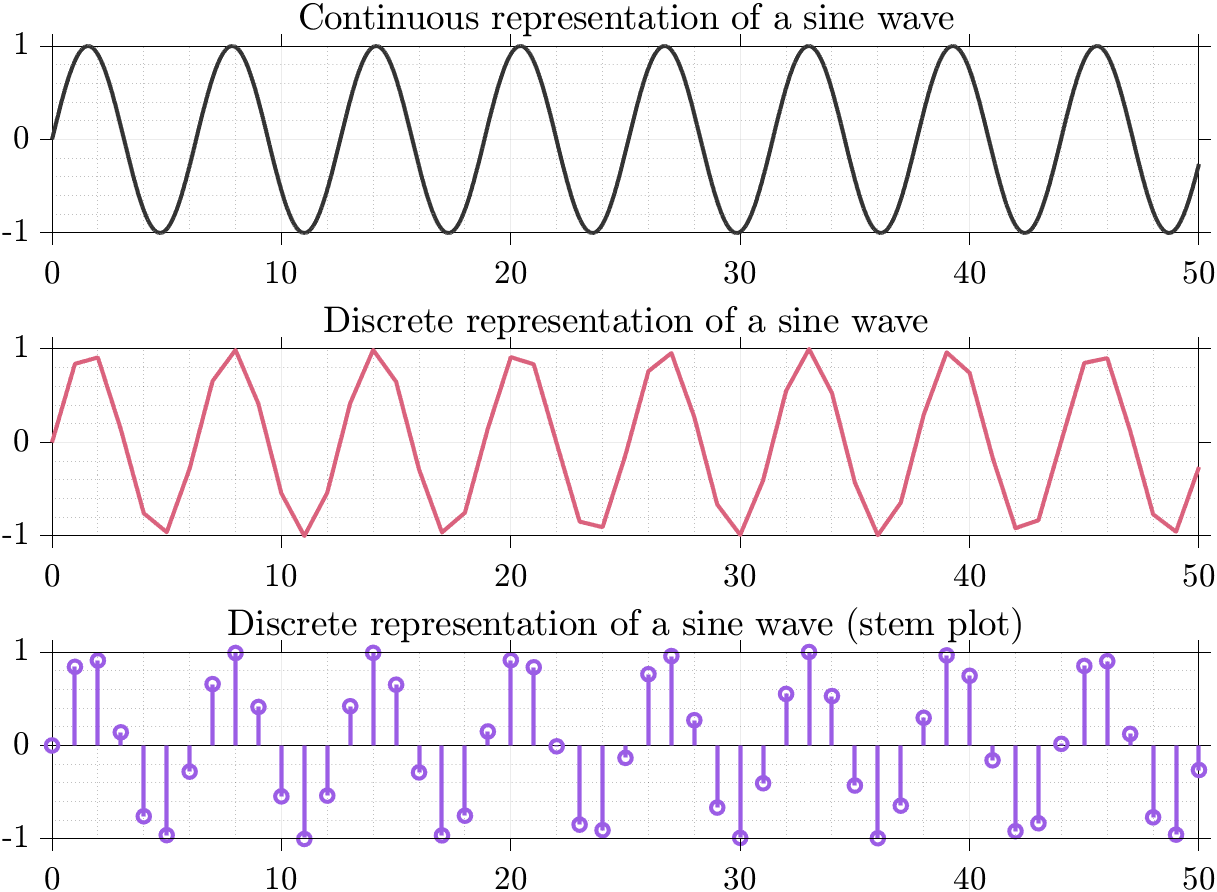
\includegraphics[width=0.55\linewidth, trim=0 0 0 0cm,clip]{figures/sampled_sine_wave.png} $x[n] = x(nT_s)$,
$T_s$ = sample time.
    
    \tiny
    Code for the figure: \url{https://github.com/rahulbhadani/CPE381_FA25/blob/main/Code/sampled_sine_wave.m}
\end{frame}

\begin{frame}{Inherent Discrete Time Signals}
    \begin{center}
         \textbf{Nature may be continuous but human activities naturally lead to some discrete time signals.} 
    \end{center}
   
    
    Examples:
    \begin{itemize}
        \item Stock market closing data
        \item Adaptive cruise control states
        \item Thermostat setpoints
    \end{itemize}
\end{frame}

%%%%%%%%%%%%%%%%%%%%%%%%%%%%%%%%%%%%%%%%%%%%%%%%%%%%%
\section{Mathematical Preliminaries}

%-----------------------------------------

\begin{frame}{}
    \begin{center}
    \Huge \bf \color{DarkBlue}
    \faCalculator
    
    Mathematical Preliminaries
\end{center}
\end{frame}

%-----------------------------------------
\begin{frame}{Trigonometry}
  \begin{columns}[T]
    \begin{column}{0.5\textwidth}
      \begin{itemize}
        \item \textbf{Sine, Cosine, Tangent:}
          \begin{itemize}
            \item \(\sin(\theta) = \cfrac{\text{p}}{\text{h}}\)
            \item \(\cos(\theta) = \cfrac{\text{b}}{\text{h}}\)
            \item \(\tan(\theta) = \cfrac{\text{p}}{\text{b}}\)
          \end{itemize}
        \item \textbf{Pythagorean Identity:}
          \[
          \sin^2(\theta) + \cos^2(\theta) = 1
          \]
      \end{itemize}
    \end{column}
    \begin{column}{0.5\textwidth}
    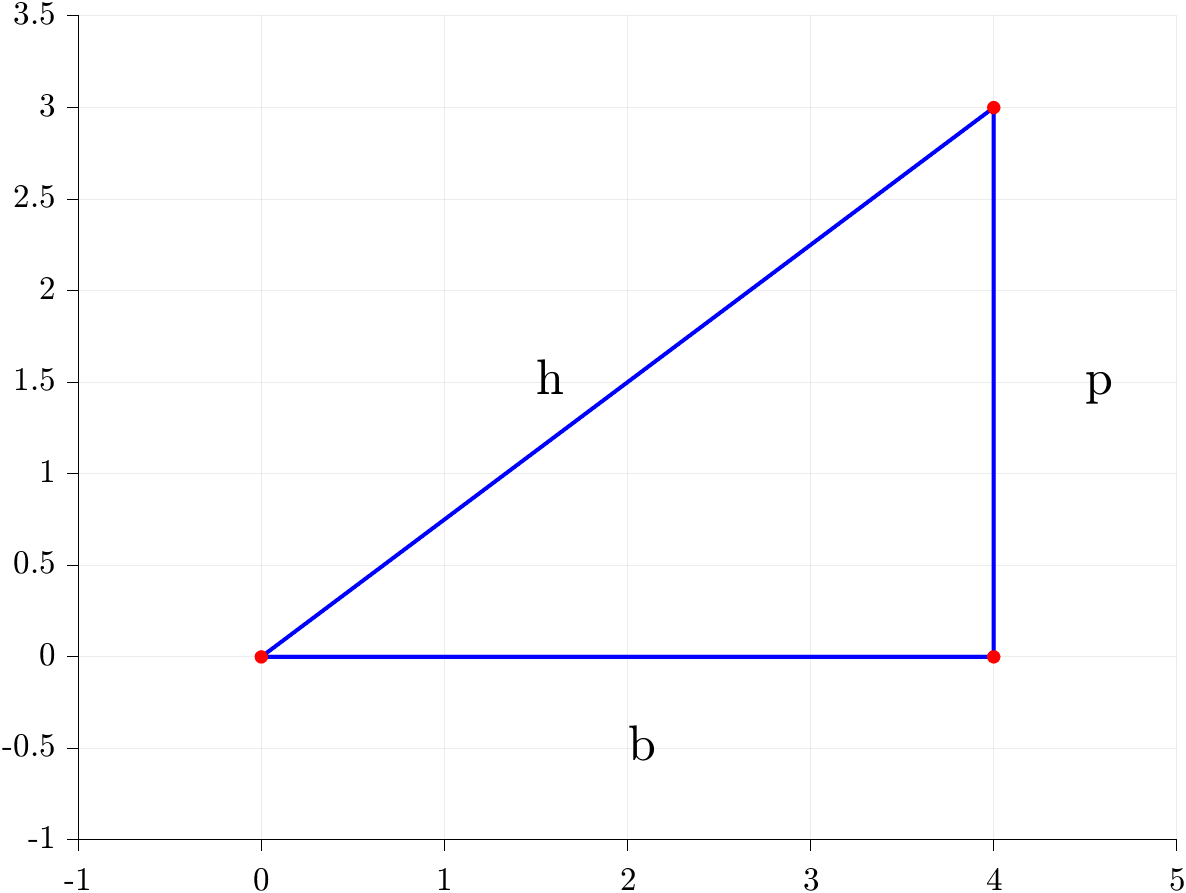
\includegraphics[width=0.60\linewidth, trim=2cm 2cm 0 0cm,clip]{figures/pythogoreas.png}
      \begin{itemize}
        \item \textbf{Unit Circle:}
      \end{itemize}
    \end{column}
  \end{columns}
\end{frame}

%-----------------------------------------
\begin{frame}{Trigonometric Identities}
What is the value of $h$ based on the diagram?
    \begin{columns}
        \column{0.3\linewidth}
 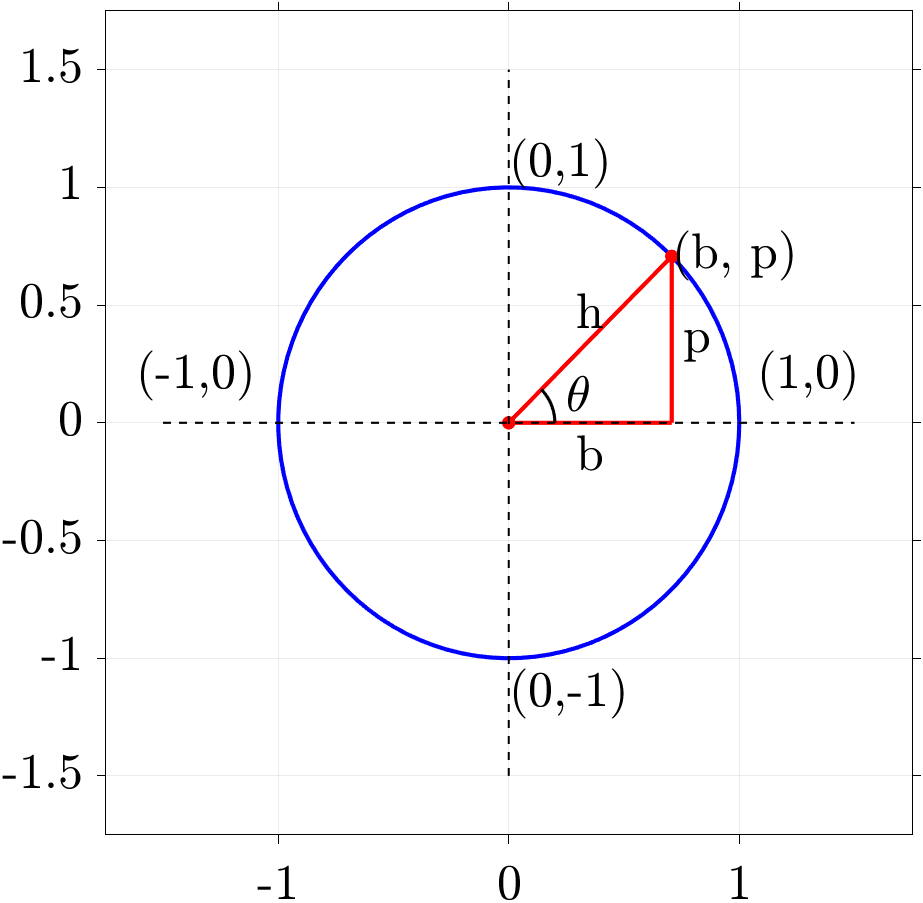
\includegraphics[width=0.99\linewidth, trim=2cm 2cm 1cm 1cm,clip]{figures/unit_circle_right_triangle.png}
         \column{0.7\linewidth}
        \begin{itemize}
            \item $\cos\theta =  $
            \item $\sin\theta = $
            \item $\sin(\alpha + \beta) = $
            \item $\cos(\alpha + \beta) = $
             \item $\sin^2(\theta) = $ $\quad\quad\quad$ in terms of $\cos(2\theta)$
              \item $\cos^2(\theta) = $ $\quad\quad\quad$ in terms of $\cos(2\theta)$
              \item $\sin 2\theta = $ $\quad\quad\quad$ in terms of $\theta$
              \item $\cos 2\theta = $ $\quad\quad\quad$ in terms of $\theta$
              \item $\sin (-\theta) = $
              \item $\cos(-\theta) = $
              
            
        \end{itemize}
    \end{columns}
\end{frame}

%-----------------------------------------
\begin{frame}{Trigonometric Identities}
What is the value of $h$ based on the diagram?
    \begin{columns}
        \column{0.3\linewidth}
 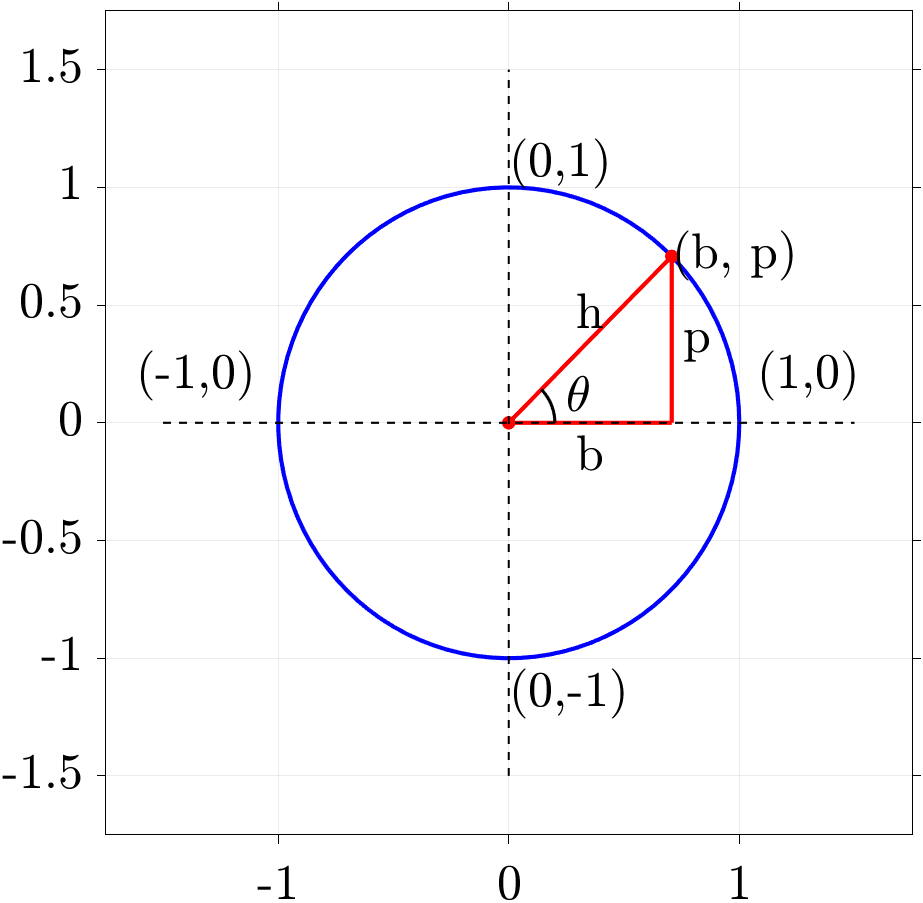
\includegraphics[width=0.99\linewidth, trim=2cm 2cm 1cm 1cm,clip]{figures/unit_circle_right_triangle.png}
         \column{0.3\linewidth}
        \begin{itemize}
            \item $\tan(\alpha + \beta) = $

             \item $\tan(\alpha - \beta) = $

              \item $\sin 30^{\circ} = $
            \item $\sin 45^{\circ} = $
            \item $\sin 60^{\circ} = $

             \end{itemize}
\column{0.3\linewidth}
 \begin{itemize}
              \item $\cos 30^{\circ} = $
            \item $\cos 45^{\circ} = $
            \item $\cos=60^{\circ} = $

               \item $\tan 30^{\circ} = $
            \item $\tan 45^{\circ} = $
            \item $\tan=60^{\circ} = $
            
        \end{itemize}
    \end{columns}

\bf \centering
    What's the range of $\sin \theta$ and $\cos \theta$?
\end{frame}

%-----------------------------------------
\begin{frame}{Trigonometric Functions in Different Quadrant}
\begin{columns}
    \column{0.4\linewidth}
    Four Quadrants:
      
        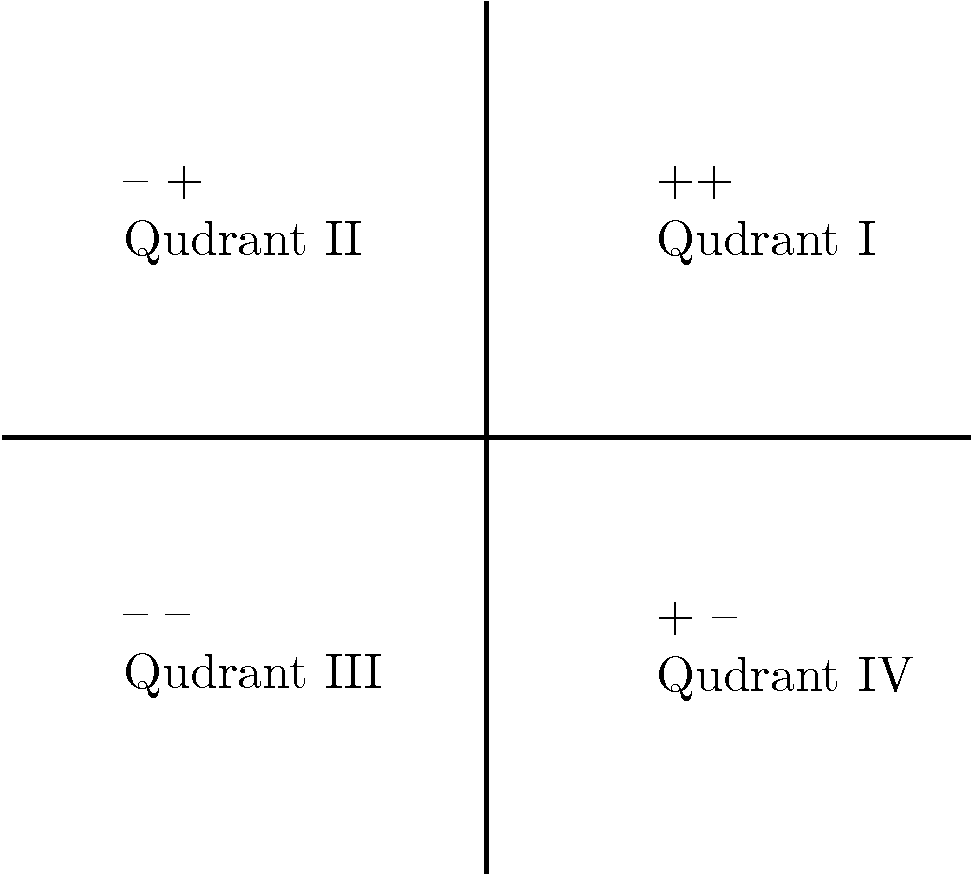
\includegraphics[width=0.99\linewidth, trim=0cm 0cm 0cm 0cm,clip]{figures/quadrants_plot.pdf}
   \column{0.6\linewidth}
   
Considering a unit circle, in four different quadrants $(x, y)$ signs are different, Hence the trigonometric ratios are also different in signs.

\begin{table}[h!]
\centering
\begin{tabular}{|c|c|c|c|}
\hline
Quadrant & $\sin$ & $\cos$ & $\tan$ \\
\hline
I & + & + & + \\
\hline
II & + & - & - \\
\hline
III & - & - & + \\
\hline
IV & - & + & - \\
\hline
\end{tabular}
\caption{Signs of $\sin$, $\cos$, and $\tan$ in all four quadrants}
\end{table}


\end{columns}
    
\end{frame}

%-----------------------------------------

\begin{frame}{Complex Number}
 \begin{columns}
        \column{0.3\linewidth}
$$z = x +  i y$$
$$ i^2  = -1$$
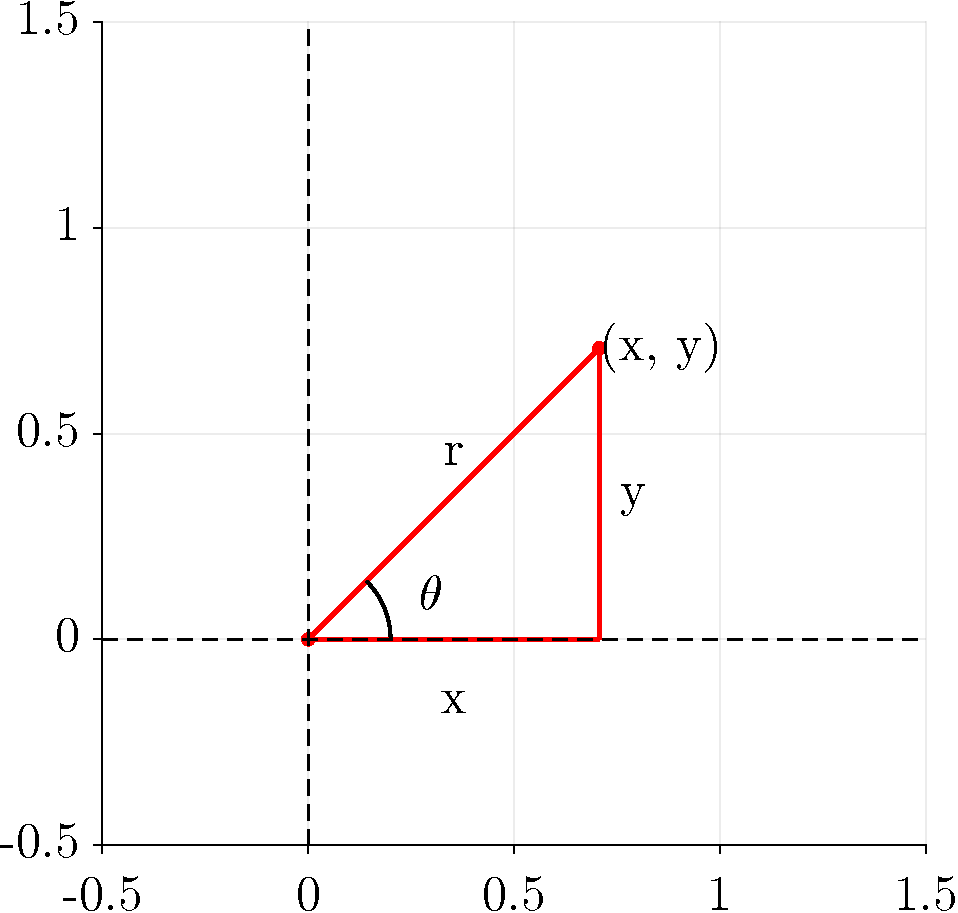
\includegraphics[width=0.99\linewidth, trim=2cm 2cm 1cm 1cm,clip]{figures/complex_num.pdf}
\column{0.3\linewidth}
Two representations of complex numbers:
$$
z = re^{i\theta}
$$
$$
\text{Conjugate:~~~} \zbar = re^{-i\theta}
$$
\column{0.4\linewidth}
    \begin{itemize}
        \item $ r = \sqrt{x^2 + y^2}$
        \item $\theta = \tan ^{-1} \cfrac{y}{x}$
    \end{itemize}
    Euler's Identity:
    \begin{itemize}
        \item $e^{i\theta} = \cos \theta + i \sin \theta$
        \item $e^{- i\theta} = $
        \item $\cos \theta  = \quad\quad\quad\quad$\\ (in terms of exponential)
        \item $\sin \theta  = \quad\quad\quad\quad$\\ (in terms of exponential)
    \end{itemize}
\end{columns}
\end{frame}

%-------------------------------------------
\begin{frame}{Complex Number}
\begin{columns}
\column{0.4\linewidth}
\textbf{Properties of Conjugates}
\begin{itemize}
    \item $\overline{z + w} = \zbar + \wbar $
    \item$ \overline{zw} = \zbar \wbar$
    \item$ \overline{z^n} = \zbar^n $
    \item $z \zbar =  | z | ^2 $ {\bf \color{red} Prove it!}
\end{itemize}
\column{0.5\linewidth}
{\bf De Moivre’s Theorem}
If $z = r(\cos \theta + i \sin \theta )$ and $n$  is a positive integer, then 
$$
z^n = [ r ( \cos \theta   + i \sin \theta  ) ^n] = r^n  ( \cos n \theta + i \sin n \theta ) 
$$

{\bf Roots of a complex number }
$z = 0$ has $n$ distinct roots:

$$
w_k =  r^{1/n}\bigg[ \cos\bigg( \cfrac{\theta + 2 k \pi }{n} \bigg)  + i \sin\bigg( \cfrac{\theta + 2 k \pi }{n} \bigg)\bigg]
$$

\end{columns}
    
\end{frame}

%-----------------------------------------
\begin{frame}{Complex Exponentials}
We also need to give a meaning to the expression $e^z$ when $z = x + i y $ is a complex number.

Based on the infinite series using Taylor's series expansion for $e^x$, we have

\begin{gradbox}{}
   $$
e^z = \sum_{n = 0}^\infty \cfrac{z^n}{n!} = 1 + z + \cfrac{z^2}{2!}  + \cfrac{z^3}{3!} + \cdots 
$$ 
\end{gradbox}

Can you find out, what should be the value of $e^{iy}$ where $y$ is the real number?

\textbf{Note: } $\cos y = 1 - \cfrac{y^2}{2!} + \cfrac{y^4}{4!} - \cfrac{y^6}{6!}  + \cdots $ and $\quad $ $\sin y =  y - \cfrac{y^3}{3!} + \cfrac{y^5}{5!} - \cdots $

    
\end{frame}


\section{Infinite Series}


\begin{frame}{}
    \begin{center}
    \Huge \bf \color{DarkBlue}
    \faFire
    
    Infinite Series
\end{center}
\end{frame}


\begin{frame}{Sum of an Infinite Sequence}
An infinite series is the sum of an infinite sequence of numbers:
$$a_1 + a_2 + a_3 + \cdots + a_n + \cdots$$
The goal is to understand the meaning of such an infinite sum and develop methods to calculate it.
\end{frame}

\begin{frame}{Partial Sums}
The $n$-th partial sum is:
$$S_n = a_1 + a_2 + a_3 + \cdots + a_n$$
As $n$ gets larger, the partial sums get closer to a limiting value.
\end{frame}

\begin{frame}{Example 1}
Consider the series:
$$1 + \frac{1}{2} + \frac{1}{4} + \frac{1}{8} + \frac{1}{16} + \cdots$$
The partial sums are:
$$S_1 = 1$$
$$S_2 = 1 + \frac{1}{2} = \frac{3}{2}$$
$$S_3 = 1 + \frac{1}{2} + \frac{1}{4} = \frac{7}{4}$$
$$S_n = 1 + \frac{1}{2} + \frac{1}{4} + \cdots + \frac{1}{2^{n-1}} =  \frac{2^n - 1}{2^{n-1}}$$
\end{frame}

\begin{frame}{Convergence of the Series}

$$
S = \lim_{n \to \infty} S_n = \lim_{n\to \infty} \cfrac{2^n - 1}{2^{n-1}} =   \lim_{n \to \infty} \bigg (  \cfrac{2^n}{2^{n-1}} - \cfrac{1}{2^{n-1}}\bigg) =  \lim_{n \to \infty} \bigg( 2 - \cfrac{1}{2^{n-1}}\bigg) 2
$$

Since the sequence of partial sums converges, the infinite series converges. That is to say:

$$\sum_{n=1}^{\infty} \frac{1}{2^{n-1}} = 2$$
\end{frame}

\begin{frame}{Arithmetic Progression (AP)}
An artihmetic series is of the form: $a, (a+d), (a+2d), \cdots (a+(n-1)d)$.

The sum can be written as:

$$
S_n = a + (a+d)  + (a+2d) + \cdots +(a + (n-1)d) = \cfrac{n}{2}[2a + (n-1)d]
$$

$
a = \text{The first term}
$, $ d = \text{common difference}$.
\end{frame}


\begin{frame}{Geometric Series/Geometric Progression}
A geometric series is of the form: $a, ar, ar^2, \cdots ar^n$.

The sum can be written as:


$$S_n = a + ar + ar^2 + ar^3 + \cdots + ar^n + \cdots = \sum_{n=1}^{\infty} ar^{n-1} = \sum_{n=0}^{\infty} ar^n$$

$
a = \text{The first term}
$, $ r = \text{common ratio}$.


\end{frame}

\begin{frame}{Convergence of Geometric Series}
If $|r| < 1$, the geometric series converges:
$$\sum_{n=1}^{\infty} ar^{n-1} = \frac{a}{1 - r}$$
If $|r| \geq 1$, the series diverges.
\end{frame}

\begin{frame}{Example 2}
Consider the series:
$$\sum_{n=0}^{\infty} (-1)^n \frac{5}{4^n}$$
This is a geometric series with $a = 5$ and $r = -\frac{1}{4}$. Since $|r| < 1$, the series converges:
$$\sum_{n=1}^{\infty} 5 \left(-\frac{1}{4}\right)^{n-1} = \frac{5}{1 - \left(-\frac{1}{4}\right)} = 4$$
\end{frame}

\begin{frame}{Example 3: Telescoping Series}
Find the sum of the telescoping series:
$$\sum_{n=1}^{\infty} \frac{1}{n(n+1)} = \sum_{n=1}^{\infty} \left(\frac{1}{n} - \frac{1}{n+1}\right)$$
The partial sums are:
$$S_n = 1 - \frac{1}{n+1} \to 1 \text{ as } n \to \infty$$
\end{frame}

\begin{frame}{Theorem}
If the series $\sum_{n=1}^{\infty} a_n$ converges, then $\lim_{n \to \infty} a_n = 0$.
\end{frame}

\begin{frame}{Divergence Test}
The series $\sum_{n=1}^{\infty} a_n$ diverges if $\lim_{n \to \infty} a_n$ fails to exist or is different from zero.
\end{frame}

\begin{frame}{Practice Problems}
Determine whether the following series converge or diverge. In the case of convergence, give the sum of the series.
\begin{enumerate}
    \item $\sum_{n=1}^{\infty} \frac{1}{2^n}$
    \item $\sum_{n=1}^{\infty} \frac{n+1}{2n-3}$
    \item $\sum_{n=2}^{\infty} \frac{n^2}{n^2-1}$
    \item $\sum_{n=1}^{\infty} \frac{n(n+2)}{(n+3)^2}$
    \item $\sum_{n=1}^{\infty} \frac{1+2n}{3^n}$
\end{enumerate}
\end{frame}



%-----------------------------------------

\begin{frame}{Derivatives}

\begin{center}
\bf
    Rate of change of a quantity with respect to another quantity.


\par In signals and systems, we are usually interested in the rate of change with respect to time.

$$
f'(t) = \cfrac{df(t)}{dt} = \lim_{h \to 0}\cfrac{f(t+h) - f(t)}{h}
$$

\begin{gradbox}{}
    In computer implementation, $h$ is $\Delta t$. $\Delta t$ is the difference of timestamps between two consecutive samples of a signal. 
\end{gradbox}
\end{center}
\end{frame}

%-----------------------------------------

\begin{frame}{Derivative Review}
 \begin{columns}
\column{0.2\linewidth}
\begin{itemize}
        
    \item $f'(x) = \cfrac{d f(x)}{dx}$
    \item $f'(t) = $
\end{itemize}

\column{0.4\linewidth}
\begin{itemize}
    \item $\frac{d}{dx}(x^n) = nx^{n-1}$
    \item $\frac{d}{dx}(\ln(x)) = \frac{1}{x}$
    \item $\frac{d}{dx}(e^x) = e^x$
    \item $\frac{d}{dx}(\sin(x)) = \cos(x)$
    \item $\frac{d}{dx}(\cos(x)) = -\sin(x)$
    \item $\frac{d}{dx}(\sin^{-1}(x)) = \frac{1}{\sqrt{1 - x^2}}$
    \item $\frac{d}{dx}(\tan(x)) = \sec^2(x)$
    \item $\frac{d}{dx}(\cot(x)) = -\csc^2(x)$
    \end{itemize}


\column{0.4\linewidth}
\begin{itemize}
\item $\frac{d}{dx}(\sec^{-1}(x)) = \frac{1}{x\sqrt{x^2 - 1}}$
    \item $\frac{d}{dx}(\sec(x)) = \sec(x) \tan(x)$
    \item $\frac{d}{dx}(\csc(x)) = -\csc(x) \cot(x)$
    \item $\frac{d}{dx}(\tan^{-1}(x)) = \frac{1}{x^2 + 1}$
    \item $(F \cdot S)' = F \cdot S' + F' \cdot S$
    \item $\left(\frac{N}{D}\right)' = \frac{D \cdot N' - N \cdot D'}{D^2}$
    \item $[f(g(x))]' = f'(g(x)) \cdot g'(x)$
\end{itemize}
\end{columns}
\end{frame}

\begin{frame}{Geometrical Interpretation of Derivatives}
\begin{center}
    \bf
    The derivative $f'(x) $ can be interpreted as the slope of the tangent line at the point $(x,y)$ on the graph of the function  $y = f(x)$.
    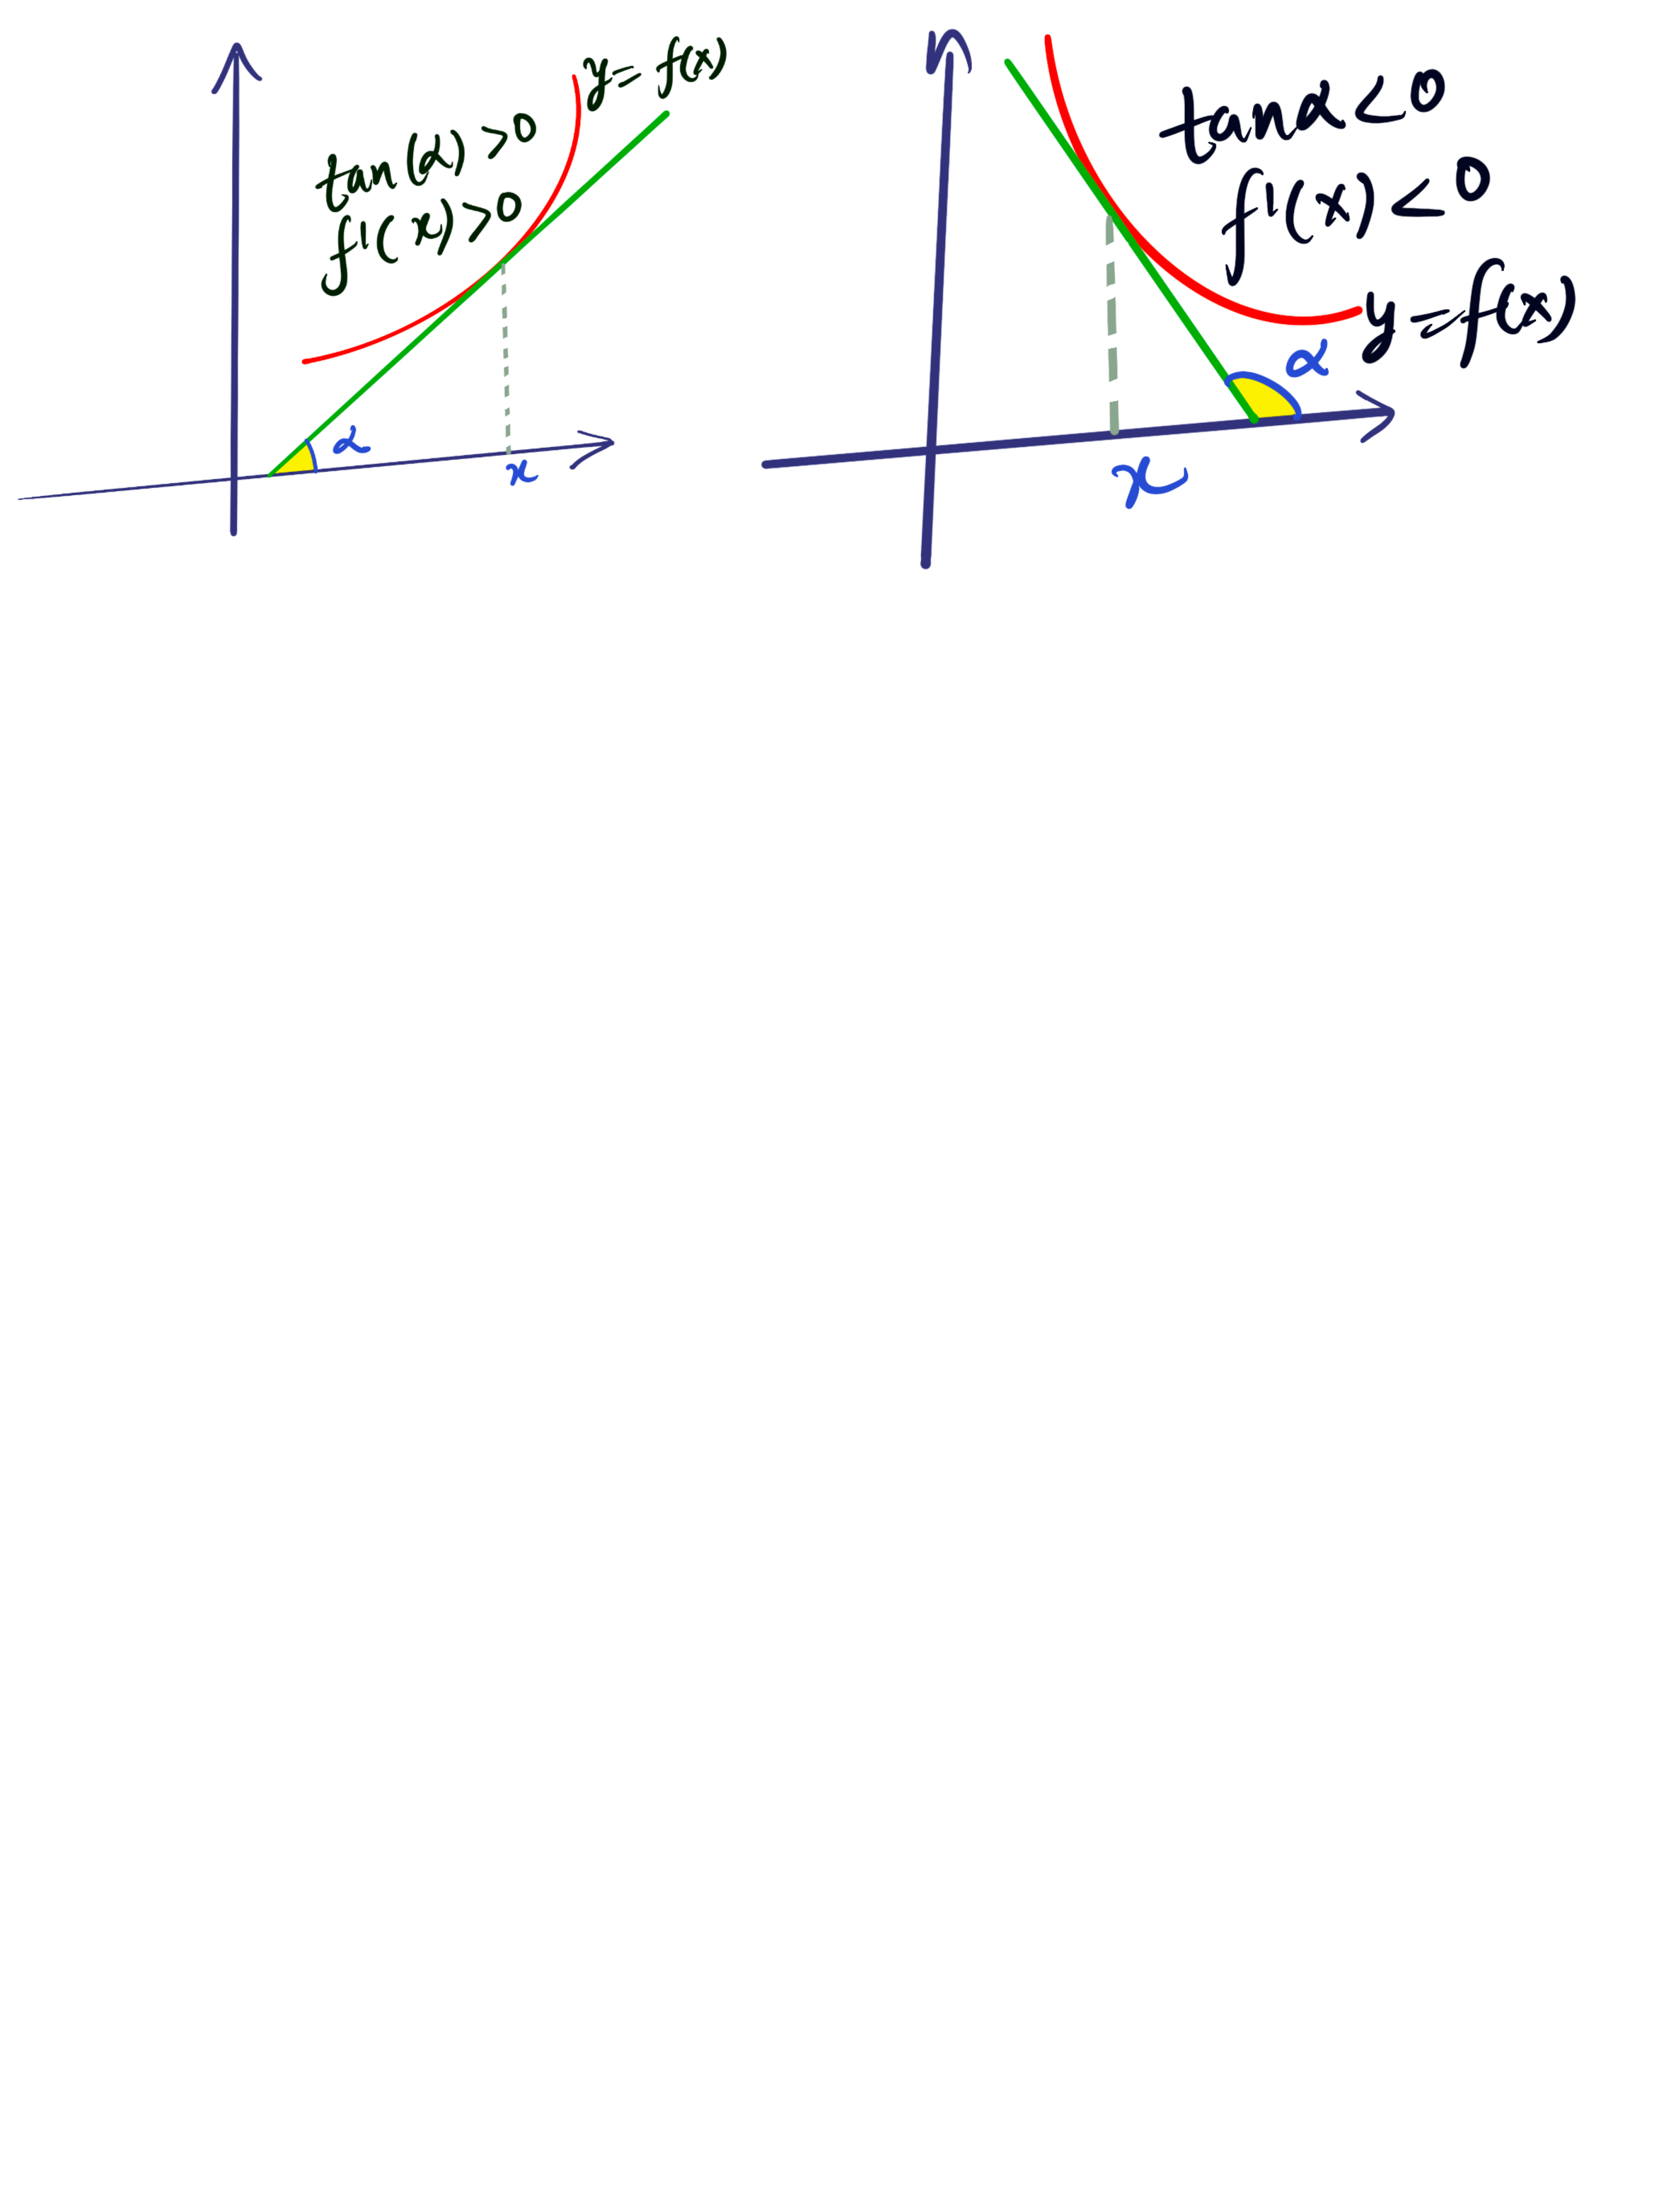
\includegraphics[width=0.99\linewidth, trim=0cm 40cm 0cm 0cm,clip]{figures/derivative.pdf}
\end{center}
\end{frame}

\begin{frame}{Geometrical Interpretation of Derivatives}
\begin{center}
    \bf We can use the geometric interpretation \\to help study the behavior and the graph of $f(x)$.
\end{center}
\begin{itemize}
    \item $f'(x) > 0$ exactly when $f(x)$ is increasing.
    \item $f'(x) < 0$ exactly when $f(x)$ is decreasing.
    \item $f'(x) = 0$ exactly when $f(x)$ has a horizontal tangent.
    \end{itemize}
\hrule \vspace{5pt}
\small
In many applications, we want to find local maximum and local minimum values. In these applications, it makes sense to look at the locations on a graph where the slope is $0$. In other words, we often use the following method to find all locations where
the slope of the graph is 0.
\begin{itemize}
    \item Find the formula for the derivative: $f'(x)$.
    \item Set this formula equal to $0$ and solve for $x$.
\end{itemize}
\end{frame}



\begin{frame}{Taylor Series}
\textbf{Function approximation:}
\[
f(x) = f(a) + f'(a)(x-a) + \frac{f''(a)}{2!}(x-a)^2 + \cdots
\]

When $a = 0$, the series is called Maclaurin series.

\textbf{Signal processing examples:}
\begin{align*}
e^x &= 1 + x + \frac{x^2}{2!} + \frac{x^3}{3!} + \cdots \\
\cos(\omega t) &= 1 - \frac{(\omega t)^2}{2!} + \frac{(\omega t)^4}{4!} - \cdots \\
\ln(1+t) &= t - \frac{t^2}{2} + \frac{t^3}{3} - \cdots \quad (|t|<1)
\end{align*}


\end{frame}


\begin{frame}{Taylor Series Applications}
\textbf{Small-angle approximation:} \\
$\sin\theta \approx \theta - \frac{\theta^3}{6}$ for $\theta \ll 1$ \\
Error at $\theta=0.1$ rad: $| \text{Actual} - \text{Approx} | < 0.001\%$

\vspace{20pt}

\textbf{Nonlinear system analysis:} \\
$y(t) = e^{x(t)} \approx 1 + x(t) + \frac{x^2(t)}{2}$ \\
When $x(t) = 0.2\cos(2\pi f t)$, \\
$y(t) \approx 1 + 0.2\cos(2\pi f t) + 0.02\cos^2(2\pi f t)$
\end{frame}



\begin{frame}{Integration}
\begin{center}
    \bf 
    Integration is antiderivative but you can also understand it as an area under the curve. In other words, integration is the summation.
\end{center}

If $\cfrac{d}{dx}F(x) = f(x)$ then $\bigints f(x) dx = F(x)$. 
    
\end{frame}

\begin{frame}{Geometric Interpretation of Integral}
    \begin{center}
        Integral gives the area under a curve
        
        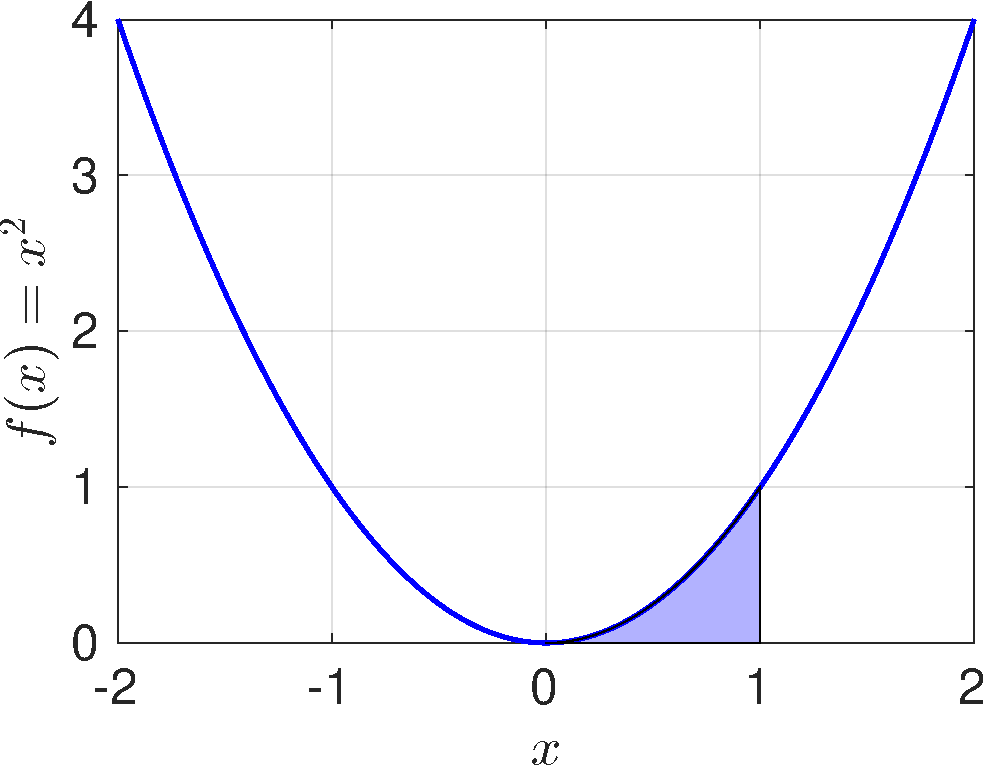
\includegraphics[width=0.29\linewidth, trim=0cm 0cm 0cm 0cm,clip]{figures/integration.pdf}

        $\int_0^1 x^2 dx$
        
    \end{center}
    
\end{frame}


%------------------------------------------------
\begin{frame}{Table of Integrals: Basic Form}

\begin{itemize}
    \item $\int x^n \, dx = \frac{1}{n+1} x^{n+1}$
    \item $\int \frac{1}{x} \, dx = \ln x$
    \item $\int u \, dv = uv - \int v \, du$
    \item $\int u(x)v'(x) \, dx = u(x)v(x) - \int v(x)u'(x) \, dx$
\end{itemize}
    
\end{frame}


\begin{frame}{Table of Integrals: More Functions}
\begin{columns}
    \column{0.5\linewidth}
    \begin{itemize}
    \item $\int \frac{1}{ax + b} \, dx = \frac{1}{a} \ln(ax + b)$
    \item $\int \frac{1}{(x + a)^2} \, dx = -\frac{1}{x + a}$
    \item $\int (x + a)^n \, dx = \frac{(x + a)^{n+1}}{n+1}, \quad n \neq -1$
    \item $\int x(x + a)^n \, dx = \frac{(x + a)^{n+1}(nx + x - a)}{(n+2)(n+1)}$
    \item $\int \frac{dx}{1 + x^2} = \tan^{-1} x$
    \item $\int \frac{dx}{a^2 + x^2} = \frac{1}{a} \tan^{-1} \left(\frac{x}{a}\right)$
    \item $\int \frac{x \, dx}{a^2 + x^2} = \frac{1}{2} \ln(a^2 + x^2)$
    \item $\int \frac{x^2 \, dx}{a^2 + x^2} = x - a \tan^{-1} \left(\frac{x}{a}\right)$
\end{itemize}

\column{0.5\linewidth}
\begin{itemize}
     
    \item $\int \frac{x^3 \, dx}{a^2 + x^2} = \frac{1}{2} x^2 - \frac{1}{2} a^2 \ln(a^2 + x^2)$
    \item $\int e^{ax} = \cfrac{1}{a}e^{ax}$
    \item $\int \sin x dx = -\cos x$
    \item $\int \cos x dx = \sin x$
    \item $\int \tan x dx = -\ln \cos x$
    
\end{itemize}
\end{columns}
\end{frame}

\begin{frame}{Differential Equations}
    \begin{center}
        \bf
        Differential equations are simply equations that have derivatives in them.
    \end{center}
Example:
\begin{itemize}
    \item $\cfrac{dy}{dx} +  5 y = 0$
    \item $y'' + 2y' + 10 y  = 0$
    \item $y'' + 3y' + 2y = 3\cos t$
    
\end{itemize}
    The order of a differential equation is the order of the highest derivative in the equation. They are all examples of `ordinary differential equations'.
\end{frame}


\begin{frame}{Solving Differential Equations}
    Consider 
    $$
    y' = 2y + 3
    $$
    The Fundamental Theorem of Calculus implies $y(t) = \int y'(t) dt$, so we get

    $$
    y(t) = 2\int y(t) dt + 3t + C
    $$
    This is not the closed form and doesn't entirely solve to find a solution $y$. We look at some formula (and their derivation) using the rules of differentiation on how to get a closed-form solution.
\end{frame}

\begin{frame}{Solving Differential Equations}
    The linear differential equation 
    $$
    y' = ay + b
    $$
    with $ a \neq 0, b$ has infinitely many solutions 
    $$
    y(t)= c e^{at}  - \cfrac{b}{a}
    $$
    \bf Proof discussed in class.
    
    \end{frame}

\begin{frame}{Up Next}
\begin{itemize}
    \item Representation of Signals: Continuous and Discrete
    \item Continuous Signals
    \item Using MATLAB
\end{itemize}
    
\end{frame}


%-----------------------------------------
\end{document}